\chapter{Theoretical Background}
\label{chapter:theoretical_background}

This chapter introduces the theoretical background that motivates the search presented in this thesis.
The discussion begins with the SM, which successfully describes a wide range of experimental observations of elementary particles and their interactions.
The limitations of the SM are then summarised, including the anomalies observed in semileptonic $B$-meson decays.
Finally, several possible extensions of the SM are introduced.
Among them, quark--lepton unification predicts leptoquarks, which connect the quark and lepton sectors directly and can explain these anomalies.
The leptoquark models are discussed in detail in Chapter~\ref{chapter:LQ_search}.

\section{The Standard Model}
\label{sec:sm}

The SM is a relativistic quantum field theory describing the known elementary particles and their strong, weak, and electromagnetic interactions. 
Its structure is determined by local gauge invariance under
\begin{align*}
    SU(3)_{C} \times SU(2)_{L} \times U(1)_{Y}.
\end{align*}
The group $SU(3)_{C}$ describes the colour symmetry of the strong interaction, while $SU(2)_{L} \times U(1)_{Y}$ describes the electroweak interaction~\cite{Glashow1961,Weinberg1967,Salam1968}. 
In quantum field theory, particles are classified by their spin and their transformation properties under the gauge symmetries. 
Particles with half-integer spin are fermions and obey Fermi--Dirac statistics, while particles with integer spin are bosons and obey Bose--Einstein statistics~\cite{Pauli1940}. 
The matter particles of the SM are spin-$1/2$ fermions, the interaction carriers are spin-$1$ gauge bosons, and the Higgs boson is a spin-$0$ scalar boson.

Since the SM Lagrangian is fixed by the field content and by the requirement of local gauge invariance, this section first summarises the field content and gauge quantum numbers of the SM. The principle of local gauge invariance is then introduced, and the covariant derivative and field-strength tensors of the SM gauge group are constructed from it, leading to the full SM Lagrangian.
Finally, electroweak symmetry breaking and the generation of fermion masses are discussed.


\subsection{Particle content and gauge group of the SM}
\label{subsec:sm_particle_content}

The gauge quantum numbers of a field specify how it transforms under the SM gauge group. 
In this thesis, the electric charge is written as
\begin{align}
    Q = T^{3} + Y,
    \label{eq:electric_charge_relation}
\end{align}
where $T^{3}$ is the third component of weak isospin and $Y$ is the weak hypercharge.

For each generation, the SM fermions are arranged as
\begin{align*}
    Q_{L}^{i}
    =
    \begin{pmatrix}
        u_{L}^{i} \\
        d_{L}^{i}
    \end{pmatrix}
    &\sim
    (3,2,1/6),
    &
    u_{R}^{i}
    &\sim
    (3,1,2/3),
    &
    d_{R}^{i}
    &\sim
    (3,1,-1/3),
    \\
    L_{L}^{i}
    =
    \begin{pmatrix}
        \nu_{L}^{i} \\
        e_{L}^{i}
    \end{pmatrix}
    &\sim
    (1,2,-1/2),
    &
    e_{R}^{i}
    &\sim
    (1,1,-1),
\end{align*}
where $i=1,2,3$ is the generation index, and the notation denotes the representation under
$SU(3)_{C}\times SU(2)_{L}\times U(1)_{Y}$, with the three entries giving the representation under the colour group of quantum chromodynamics~(QCD), the weak isospin representation and the weak hypercharge, respectively.
In the SM, no right-handed neutrino field is included. 
The scalar sector contains one complex Higgs doublet,
\begin{align*}
    \Phi
    =
    \begin{pmatrix}
        \phi^{+} \\
        \phi^{0}
    \end{pmatrix}
    \sim
    (1,2,1/2).
\end{align*}

The gauge bosons are associated with the generators of the three gauge groups. 
The eight gluon fields $G_{\mu}^{a}$, with $a=1,\ldots,8$, are associated with $SU(3)_{C}$. 
The three weak gauge fields $W_{\mu}^{I}$, with $I=1,2,3$, are associated with $SU(2)_{L}$. 
The hypercharge gauge field $B_{\mu}$ is associated with $U(1)_{Y}$. 
Before electroweak symmetry breaking, $W_{\mu}^{1}$, $W_{\mu}^{2}$, $W_{\mu}^{3}$, and $B_{\mu}$ are gauge eigenstates. 
After electroweak symmetry breaking, they are reorganised into the physical electroweak bosons $W^{\pm}$, $Z$, and $\gamma$.

The particle content of the SM is summarised in Table~\ref{tab:sm_particles}. 
For fermions and the Higgs boson, the table lists the corresponding electroweak quantum numbers using the convention in Eq.~\eqref{eq:electric_charge_relation}. 
For gauge bosons, the table lists their spins and electric charges.

\begin{table}[htbp]
    \centering
    \caption[Standard Model particle content]{
    Particle content of the SM and the corresponding spin and electroweak quantum numbers.
    }
    \label{tab:sm_particles}
    \scriptsize
    \resizebox{\textwidth}{!}{
    \begin{tabular}{ccccccccc}
        \toprule
        \multirow{2}{*}{Category}
        & \multirow{2}{*}{Type}
        & \multicolumn{3}{c}{Generation}
        & \multirow{2}{*}{Spin}
        & \multicolumn{3}{c}{Quantum numbers} \\
        & & 1st & 2nd & 3rd & & $T^{3}$ & $Y$ & $Q$ \\
        \midrule

        \multirow{5}{*}{Fermion}
        & Left-handed quark
        & $\begin{array}{c} u_{L} \\ d_{L} \end{array}$
        & $\begin{array}{c} c_{L} \\ s_{L} \end{array}$
        & $\begin{array}{c} t_{L} \\ b_{L} \end{array}$
        & $1/2$
        & $\begin{array}{c} +1/2 \\ -1/2 \end{array}$
        & $1/6$
        & $\begin{array}{c} +2/3 \\ -1/3 \end{array}$ \\

        & Right-handed up-type quark
        & $u_{R}$
        & $c_{R}$
        & $t_{R}$
        & $1/2$
        & $0$
        & $2/3$
        & $+2/3$ \\

        & Right-handed down-type quark
        & $d_{R}$
        & $s_{R}$
        & $b_{R}$
        & $1/2$
        & $0$
        & $-1/3$
        & $-1/3$ \\

        \cmidrule(lr){2-9}

        & Left-handed lepton
        & $\begin{array}{c} \nu_{eL} \\ e_{L} \end{array}$
        & $\begin{array}{c} \nu_{\mu L} \\ \mu_{L} \end{array}$
        & $\begin{array}{c} \nu_{\tau L} \\ \tau_{L} \end{array}$
        & $1/2$
        & $\begin{array}{c} +1/2 \\ -1/2 \end{array}$
        & $-1/2$
        & $\begin{array}{c} 0 \\ -1 \end{array}$ \\

        & Right-handed charged lepton
        & $e_{R}$
        & $\mu_{R}$
        & $\tau_{R}$
        & $1/2$
        & $0$
        & $-1$
        & $-1$ \\

        \midrule

        \multirow{4}{*}{Gauge boson}
        & Gluon
        & \multicolumn{3}{c}{$g^{a}$, $a=1,\ldots,8$}
        & $1$
        & --
        & --
        & $0$ \\

        & Photon
        & \multicolumn{3}{c}{$\gamma$}
        & $1$
        & --
        & --
        & $0$ \\

        & Charged weak boson
        & \multicolumn{3}{c}{$W^{\pm}$}
        & $1$
        & --
        & --
        & $\pm1$ \\

        & Neutral weak boson
        & \multicolumn{3}{c}{$Z$}
        & $1$
        & --
        & --
        & $0$ \\

        \midrule

        Scalar field
        & Higgs doublet
        & \multicolumn{3}{c}{
            $\begin{array}{c}
                \phi^{+} \\
                \phi^{0}
            \end{array}$
        }
        & $0$
        & $\begin{array}{c} +1/2 \\ -1/2 \end{array}$
        & $1/2$
        & $\begin{array}{c} +1 \\ 0 \end{array}$ \\

        \bottomrule
    \end{tabular}
    }
\end{table}

% The quantum numbers listed above determine which interactions each field can have. 
% They also determine which terms can be written in the SM Lagrangian. 
% For example, explicit Dirac mass terms for charged fermions are not gauge invariant before electroweak symmetry breaking, because the left- and right-handed fermions transform differently under $SU(2)_{L}\times U(1)_{Y}$. 
% Fermion masses instead arise from gauge-invariant Yukawa interactions with the Higgs field.


\subsection{Local gauge invariance and the gauge interactions}
\label{subsec:local_gauge_invariance}

The interactions of the SM follow from invariance under local gauge transformations.
A field $\psi(x)$ in a representation with generators $T^{A}$ transforms as
\begin{align*}
    \psi(x)
    \rightarrow
    \psi'(x)
    =
    U(x)\psi(x),
    \qquad
    U(x)
    =
    \exp\left[i\alpha^{A}(x)T^{A}\right],
\end{align*}
where $\alpha^{A}(x)$ are arbitrary real gauge parameters that depend on $x$, and the repeated index $A$ is summed over all generators. 
Because $U(x)$ depends on $x$, the ordinary derivative $\partial_{\mu}\psi$ acquires an additional term $(\partial_{\mu}U)\psi$ and does not transform in the same way as $\psi$, so a kinetic term built from it is not gauge invariant. 
Local gauge invariance is restored by replacing $\partial_{\mu}$ with a covariant derivative
\begin{align}
    D_{\mu}
    =
    \partial_{\mu}
    -
    ig_{A}A_{\mu}^{A}T^{A},
    \label{eq:generic_covariant_derivative}
\end{align}
which introduces one gauge field $A_{\mu}^{A}$ with coupling $g_{A}$ for each generator. 
The gauge fields are chosen such that $D_{\mu}\psi$ transforms in the same way as $\psi$,
\begin{align*}
    D_{\mu}\psi(x)
    \rightarrow
    D'_{\mu}\psi'(x)
    =
    U(x)D_{\mu}\psi(x).
\end{align*}
With $A_{\mu}=A_{\mu}^{A}T^{A}$, this requirement is satisfied if the gauge fields transform as
\begin{align*}
    A_{\mu}(x)
    \rightarrow
    A'_{\mu}(x)
    =
    U(x)A_{\mu}(x)U^{\dagger}(x)
    -
    \frac{i}{g_{A}}
    \left(\partial_{\mu}U(x)\right)U^{\dagger}(x).
\end{align*}
The gauge fields are therefore not added by hand as arbitrary new particles. 
They are required in order to compare fields at neighbouring spacetime points in a way that is independent of the local gauge convention.

For the SM gauge group $SU(3)_{C}\times SU(2)_{L}\times U(1)_{Y}$, Eq.~\eqref{eq:generic_covariant_derivative} becomes
\begin{align}
    D_{\mu}
    =
    \partial_{\mu}
    -
    ig_{s}G_{\mu}^{a}T_{C}^{a}
    -
    igW_{\mu}^{I}T_{L}^{I}
    -
    ig'YB_{\mu},
    \label{eq:sm_covariant_derivative}
\end{align}
where $g_{s}$, $g$ and $g'$ are the gauge couplings of $SU(3)_{C}$, $SU(2)_{L}$ and $U(1)_{Y}$. 
Here $T_{C}^{a}=\lambda^{a}/2$ and $T_{L}^{I}=\tau^{I}/2$ are the generators acting on colour triplets and $SU(2)_{L}$ doublets, with $\lambda^{a}$ the Gell-Mann matrices and $\tau^{I}$ the Pauli matrices. 
The value of $Y$ is the hypercharge of the field. 

The gauge kinetic terms are built from the field-strength tensors
\begin{align*}
    G_{\mu\nu}^{a}
    &=
    \partial_{\mu}G_{\nu}^{a}
    -
    \partial_{\nu}G_{\mu}^{a}
    +
    g_{s}f^{abc}G_{\mu}^{b}G_{\nu}^{c},
    \\
    W_{\mu\nu}^{I}
    &=
    \partial_{\mu}W_{\nu}^{I}
    -
    \partial_{\nu}W_{\mu}^{I}
    +
    g\epsilon^{IJK}W_{\mu}^{J}W_{\nu}^{K},
    \\
    B_{\mu\nu}
    &=
    \partial_{\mu}B_{\nu}
    -
    \partial_{\nu}B_{\mu},
\end{align*}
where $f^{abc}$ and $\epsilon^{IJK}$ are the structure constants of $SU(3)_{C}$ and $SU(2)_{L}$.
The terms quadratic in the gauge fields arise because the generators of these non-Abelian groups do not commute.
When the field-strength tensors are squared in the gauge kinetic terms, they produce self-interactions among the gluons and among the $SU(2)_{L}$ gauge fields.

\subsection{The Standard Model Lagrangian}
\label{subsec:sm_lagrangian}

Using the field content, covariant derivative and field-strength tensors introduced above, the SM Lagrangian can be written as the sum of gauge-boson kinetic terms, fermion kinetic terms, the Higgs-sector terms, and Yukawa interactions. 
\begin{align}
    \mathcal{L}_{\mathrm{SM}}
    =
    \mathcal{L}_{\mathrm{gauge}}
    +
    \mathcal{L}_{\mathrm{fermion}}
    +
    \mathcal{L}_{\mathrm{Higgs}}
    +
    \mathcal{L}_{\mathrm{Yukawa}}.
    \label{eq:sm_lagrangian_decomposition}
\end{align}
The four terms in Eq.~\eqref{eq:sm_lagrangian_decomposition} are fixed by Lorentz invariance, local gauge invariance, and renormalisability, once the SM field content is specified~\cite{PDG2024}.

The gauge-boson kinetic term is
\begin{align}
    \mathcal{L}_{\mathrm{gauge}}
    =
    -
    \frac{1}{4}
    G_{\mu\nu}^{a}G^{a\mu\nu}
    -
    \frac{1}{4}
    W_{\mu\nu}^{I}W^{I\mu\nu}
    -
    \frac{1}{4}
    B_{\mu\nu}B^{\mu\nu}.
    \label{eq:sm_gauge_lagrangian}
\end{align}
The derivative terms of the field-strength tensors describe the free propagation of the gauge fields, and the terms $g_{s}f^{abc}G_{\mu}^{b}G_{\nu}^{c}$ and $g\epsilon^{IJK}W_{\mu}^{J}W_{\nu}^{K}$ give the self-interactions noted above.

The fermion kinetic terms are
\begin{align}
    \mathcal{L}_{\mathrm{fermion}}
    =
    \sum_{i=1}^{3}
    \bigg[
        &
        \bar{Q}_{L}^{i} i\gamma^{\mu}D_{\mu}Q_{L}^{i}
        +
        \bar{u}_{R}^{i} i\gamma^{\mu}D_{\mu}u_{R}^{i}
        +
        \bar{d}_{R}^{i} i\gamma^{\mu}D_{\mu}d_{R}^{i}
    \nonumber\\
        &+
        \bar{L}_{L}^{i} i\gamma^{\mu}D_{\mu}L_{L}^{i}
        +
        \bar{e}_{R}^{i} i\gamma^{\mu}D_{\mu}e_{R}^{i}
    \bigg],
    \label{eq:sm_fermion_lagrangian}
\end{align}
where $\bar{Q}_{L}^{i}=(Q_{L}^{i})^{\dagger}\gamma^{0}$ is the Dirac adjoint of $Q_{L}^{i}$, and the same definition applies to the other fermion fields.
The covariant derivative is given by Eq.~\eqref{eq:sm_covariant_derivative}. 
Therefore, Eq.~\eqref{eq:sm_fermion_lagrangian} describes both the free propagation of fermions and their gauge interactions.

The Higgs-sector terms are
\begin{align}
    \mathcal{L}_{\mathrm{Higgs}}
    =
    (D_{\mu}\Phi)^{\dagger}(D^{\mu}\Phi)
    -
    V(\Phi),
    \qquad
    V(\Phi)
    =
    -
    \mu^{2}\Phi^{\dagger}\Phi
    +
    \lambda(\Phi^{\dagger}\Phi)^{2}.
    \label{eq:sm_higgs_lagrangian}
\end{align}
The first term is the kinetic term of the Higgs doublet and also contains the gauge interactions of the Higgs field through the covariant derivative. 
The function $V(\Phi)$ is the Higgs potential. 
$\mu^{2}$ is the mass parameter of the Higgs field and $\lambda$ is the Higgs self-coupling, with $\mu^{2}>0$ and $\lambda>0$.
$\lambda>0$ makes $V(\Phi)$ rise at large $\Phi^{\dagger}\Phi$, while $\mu^{2}>0$ places the minimum at a non-zero value of $\Phi^{\dagger}\Phi$. 
This leads to electroweak symmetry breaking through the Brout--Englert--Higgs mechanism~\cite{Englert1964,Higgs1964,Guralnik1964}.

The Yukawa interactions are
\begin{align*}
    \mathcal{L}_{\mathrm{Yukawa}}
    =
    -
    y_{d}^{ij}\bar{Q}_{L}^{i}\Phi d_{R}^{j}
    -
    y_{u}^{ij}\bar{Q}_{L}^{i}\tilde{\Phi} u_{R}^{j}
    -
    y_{e}^{ij}\bar{L}_{L}^{i}\Phi e_{R}^{j}
    +
    \mathrm{h.c.},
\end{align*}
where $i,j=1,2,3$ are generation indices, and $y_{u}^{ij}$, $y_{d}^{ij}$, and $y_{e}^{ij}$ are complex Yukawa coupling matrices in flavour space. 
$\mathrm{h.c.}$ denotes the Hermitian conjugate. 
The conjugate Higgs doublet is defined as
\begin{align*}
    \tilde{\Phi}
    =
    i\tau^{2}\Phi^{*}.
\end{align*}
The field $\tilde{\Phi}$ transforms as an $SU(2)_{L}$ doublet with hypercharge opposite to that of $\Phi$, allowing a gauge-invariant Yukawa interaction for up-type quarks.

\subsection{Electroweak symmetry breaking and the Higgs mechanism}
\label{subsec:ewsb}

For the Higgs potential in Eq.~\eqref{eq:sm_higgs_lagrangian}, the minimum satisfies $\Phi^{\dagger}\Phi=v^{2}/2$, where $v=\sqrt{\mu^{2}/\lambda}$ is the Higgs vacuum expectation value and sets the electroweak scale. 
A convenient choice of vacuum expectation value is
\begin{align}
    \langle\Phi\rangle
    =
    \frac{1}{\sqrt{2}}
    \begin{pmatrix}
        0 \\
        v
    \end{pmatrix}.
    \label{eq:higgs_vev}
\end{align}
The value of $v$ is related to the Fermi constant by~\cite{PDG2024}
\begin{align*}
    v=(\sqrt{2}G_{F})^{-1/2}\simeq 246~\GeV.
\end{align*}

This vacuum breaks the electroweak symmetry according to
\begin{align*}
    SU(2)_{L}\times U(1)_{Y}
    \rightarrow
    U(1)_{\mathrm{em}}.
\end{align*}
The unbroken symmetry is electromagnetism.

In unitary gauge, the Higgs doublet can be written as
\begin{align*}
    \Phi(x)
    =
    \frac{1}{\sqrt{2}}
    \begin{pmatrix}
        0 \\
        v+h(x)
    \end{pmatrix},
\end{align*}
where $h(x)$ is the physical Higgs boson field. 
Expanding the Higgs potential around the vacuum gives
\begin{align*}
    V(\Phi)
    =
    V(\langle\Phi\rangle)
    +
    \frac{1}{2}m_{h}^{2}h^{2}
    +
    \lambda v h^{3}
    +
    \frac{\lambda}{4}h^{4},
\end{align*}
where the physical Higgs-boson mass is
\begin{align*}
    m_{h}^{2}
    =
    2\lambda v^{2}
    =
    2\mu^{2}.
\end{align*}
Unlike the $W$ and $Z$ boson masses, which are fixed at tree level by the electroweak gauge couplings and the vacuum expectation value, the Higgs-boson mass depends on the Higgs self-coupling $\lambda$. 
Therefore, the SM does not predict the numerical value of $m_{h}$ before $\lambda$ is fixed experimentally. 
The Higgs boson was observed by the ATLAS and CMS experiments in 2012~\cite{ATLAS2012Higgs,CMS2012Higgs}. 
The observed Higgs-boson mass is approximately $125~\GeV$, corresponding to $\lambda\simeq m_{h}^{2}/(2v^{2})\simeq0.13$~\cite{ATLASCMSHiggsMass2015}.

The masses of the electroweak gauge bosons arise from the kinetic term $(D_{\mu}\Phi)^{\dagger}(D^{\mu}\Phi)$ after substituting the Higgs vacuum expectation value. 
The charged weak fields are
\begin{align*}
    W_{\mu}^{\pm}
    =
    \frac{1}{\sqrt{2}}
    \left(
        W_{\mu}^{1}
        \mp
        iW_{\mu}^{2}
    \right).
\end{align*}
Substituting the vacuum expectation value from Eq.~\eqref{eq:higgs_vev} into the kinetic term of Eq.~\eqref{eq:sm_higgs_lagrangian} gives
\begin{align*}
    (D_{\mu}\langle\Phi\rangle)^{\dagger}
    (D^{\mu}\langle\Phi\rangle)
    =
    \frac{g^{2}v^{2}}{4}W_{\mu}^{+}W^{-\mu}
    +
    \frac{v^{2}}{8}
    \left(
        gW_{\mu}^{3}
        -
        g'B_{\mu}
    \right)^{2}.
\end{align*}
The first term is the mass term of the $W^{\pm}$ bosons. 
The second term shows that the neutral gauge fields $W_{\mu}^{3}$ and $B_{\mu}$ mix and must be diagonalised.

The weak mixing angle is defined by
\begin{align*}
    \cos\theta_{W}
    =
    \frac{g}{\sqrt{g^{2}+g'^{2}}},
    \qquad
    \sin\theta_{W}
    =
    \frac{g'}{\sqrt{g^{2}+g'^{2}}}.
\end{align*}
The corresponding neutral mass eigenstates are the fields of the photon and the $Z$ boson,
\begin{align*}
    A_{\mu}
    &=
    B_{\mu}\cos\theta_{W}
    +
    W_{\mu}^{3}\sin\theta_{W},
    \\
    Z_{\mu}
    &=
    -
    B_{\mu}\sin\theta_{W}
    +
    W_{\mu}^{3}\cos\theta_{W}.
\end{align*} 

The resulting gauge-boson masses are
\begin{align*}
    m_{W}
    =
    \frac{1}{2}gv,
    \qquad
    m_{Z}
    =
    \frac{1}{2}\sqrt{g^{2}+g'^{2}}\,v
    =
    \frac{m_{W}}{\cos\theta_{W}},
    \qquad
    m_{\gamma}=0.
\end{align*}
Thus, the SM predicts the relation $m_{W}=m_{Z}\cos\theta_{W}$, and inserting $v \simeq 246~\GeV$ and the electroweak couplings gives $m_{W}\simeq80~\GeV$ and $m_{Z}\simeq91~\GeV$.

The massless photon field $A_{\mu}$ is the gauge field of the unbroken $U(1)_{\mathrm{em}}$, and its interactions with charged fermions are described by quantum electrodynamics~(QED). 
For a charged fermion field $\psi$ with electric charge $Q$, the QED Lagrangian can be written as
\begin{align*}
    \mathcal{L}_{\mathrm{QED}}
    =
    -
    \frac{1}{4}
    F_{\mu\nu}F^{\mu\nu}
    +
    \bar{\psi}
    \left(
        i\gamma^{\mu}D_{\mu}
        -
        m
    \right)
    \psi,
\end{align*}
where
\begin{align*}
    D_{\mu}
    =
    \partial_{\mu}
    -
    ieQA_{\mu},
    \qquad
    F_{\mu\nu}
    =
    \partial_{\mu}A_{\nu}
    -
    \partial_{\nu}A_{\mu},
\end{align*}
where $e$ is the electromagnetic coupling and the elementary charge, $Q$ is the electric charge of the fermion in units of $e$, and $F_{\mu\nu}$ is the electromagnetic field-strength tensor.


\subsection{Fermion masses and flavour mixing}
\label{subsec:yukawa_flavour}

The Yukawa interactions generate fermion masses after electroweak symmetry breaking. 
When the Higgs field acquires its vacuum expectation value $v$, the Yukawa coupling matrices are converted into fermion mass matrices:
\begin{align*}
    M_{u}^{ij}
    =
    \frac{v}{\sqrt{2}}y_{u}^{ij},
    \qquad
    M_{d}^{ij}
    =
    \frac{v}{\sqrt{2}}y_{d}^{ij},
    \qquad
    M_{e}^{ij}
    =
    \frac{v}{\sqrt{2}}y_{e}^{ij},
\end{align*}
where $M_{u}$, $M_{d}$, and $M_{e}$ are the mass matrices of the up-type quarks, down-type quarks, and charged leptons, respectively. 
% Since the Yukawa matrices are in general not diagonal, the mass matrices are also not diagonal in the weak-interaction basis.

The physical fermion masses are obtained by diagonalising the mass matrices. 
In the quark sector, the up-type and down-type mass matrices are diagonalised by different rotations in flavour space. 
As a result, flavour mixing appears in the charged-current weak interaction. 
This mixing is described by the Cabibbo--Kobayashi--Maskawa~(CKM) matrix~\cite{Cabibbo1963,KobayashiMaskawa1973}. 
In the mass eigenstate basis, the charged-current interaction of quarks is
\begin{align*}
    \mathcal{L}_{\mathrm{CC}}
    =
    \frac{g}{\sqrt{2}}
    \bar{u}_{L}^{i}
    \gamma^{\mu}
    V_{ij}^{\mathrm{CKM}}
    d_{L}^{j}
    W_{\mu}^{+}
    +
    \mathrm{h.c.},
\end{align*}
where $u_{L}^{i}$ and $d_{L}^{j}$ are the left-handed up-type and down-type quark mass eigenstates. 
The matrix element $V_{ij}^{\mathrm{CKM}}$ describes the strength of the charged-current transition from the down-type quark $d_{L}^{j}$ to the up-type quark $u_{L}^{i}$, and the Hermitian-conjugate term describes the corresponding interaction involving $W_{\mu}^{-}$. 
The CKM matrix sets the strength of flavour-changing charged-current processes such as $b\rightarrow c\tau\nu$. 
Its complex phase also provides a source of CP violation in the quark sector of the SM.


\section{Beyond the Standard Model}
\label{sec:bsm}

Despite its success, the SM is not a complete theory of nature. 
This section summarises the experimental and theoretical facts that point to physics beyond the SM.

\subsection{Gravity and the Planck scale}
\label{subsec:gravity_planck_scale}

The SM describes the electromagnetic, weak, and strong interactions as quantum gauge field theories, but it does not include gravity. 
Gravity is instead described at macroscopic scales by general relativity. 
A complete theory of nature is therefore expected to provide a consistent quantum description of gravity and to explain its connection to the SM interactions.

The difficulty of connecting gravity with the SM appears in two related ways. 
First, quantum gravitational effects are expected to become important at the Planck scale, $M_{\mathrm{Pl}}\sim10^{19}~\GeV$. This is much higher than the electroweak scale, $v\simeq246~\GeV$.
This large separation of scales is closely related to the hierarchy problem discussed below.

Second, if general relativity is quantised perturbatively in the same way as ordinary quantum field theories, it is not renormalisable as a fundamental theory. 
Gravity therefore cannot be added to the SM in the same framework as the other interactions. 
Several possible approaches to quantum gravity have been proposed, including string theory and loop quantum gravity, although no complete theory has been experimentally confirmed.

\subsection{The hierarchy problem}
\label{subsec:hierarchy_problem}

The hierarchy problem arises because the Higgs mass parameter is highly sensitive to physics at very high energy scales. 
If the SM is treated as an effective theory valid up to an ultraviolet cutoff scale $\Lambda$, loop corrections to the Higgs mass can be written schematically as
\begin{align*}
    m_{h,\mathrm{phys}}^{2}
    =
    m_{h,0}^{2}
    +
    \delta m_{h}^{2},
\end{align*}
where $m_{h,0}^{2}$ is the bare Higgs mass parameter and $\delta m_{h}^{2}$ denotes the quantum correction. 
At one-loop order, the correction contains terms quadratically sensitive to the cutoff scale,
\begin{align*}
    \delta m_{h}^{2}
    \sim
    \frac{\Lambda^{2}}{16\pi^{2}}.
\end{align*}
If the cutoff scale is close to the Planck scale, $\Lambda\sim M_{\mathrm{Pl}}\sim10^{19}~\GeV$, the magnitude of $\delta m_{h}^{2}$ is many orders of magnitude larger than the observed value $m_{h}^{2}\sim(125~\GeV)^{2}$. 
Therefore, the bare parameter $m_{h,0}^{2}$ and the quantum correction $\delta m_{h}^{2}$ must cancel each other with extremely high precision in order to leave the observed electroweak-scale Higgs mass. 
This required cancellation is known as fine-tuning.

This fine-tuning motivates many extensions of the SM, such as supersymmetry, composite Higgs models, and other scenarios in which new physics appears near the \TeV{} scale and stabilises the Higgs mass against large ultraviolet corrections. 
The hierarchy problem is therefore one of the main motivations for searches for new particles at the \TeV{} scale. 


\subsection{Neutrino masses}
\label{subsec:neutrino_masses}

In the SM, neutrinos are massless because no right-handed neutrino fields are included and no renormalisable neutrino mass term can be written using only the SM field content. 
However, neutrino oscillation experiments have shown that neutrinos change flavour as they propagate, which requires non-zero neutrino mass differences. 
Evidence for atmospheric neutrino oscillations was reported by the Super-Kamiokande experiment~\cite{SuperK1998}, and solar neutrino flavour transformation was established by the Sudbury Neutrino Observatory~\cite{SNO2002}. 
Therefore, neutrino masses provide direct experimental evidence for physics beyond the SM.

\subsection{Dark matter}
\label{subsec:dark_matter}

Astrophysical and cosmological observations indicate the existence of non-luminous matter that cannot be explained by the known particles of the SM. 
Measurements of the cosmic microwave background, for example by the Planck satellite, are well described by a cosmological model containing a significant non-baryonic dark matter component~\cite{Planck2018}. 
The SM does not contain a suitable cold dark matter candidate. 
Although neutrinos are electrically neutral and weakly interacting, their small masses and relativistic behaviour in the early universe do not provide the required cold dark matter component.

\subsection{Matter--antimatter asymmetry}
\label{subsec:baryon_asymmetry}

The observable universe contains much more matter than antimatter. 
Sakharov identified three necessary conditions for dynamically generating such a baryon asymmetry: baryon-number violation, C and CP violation, and departure from thermal equilibrium~\cite{Sakharov1967}. 
The SM contains CP violation through the CKM matrix and baryon-plus-lepton number violation through non-perturbative electroweak effects. 
However, the amount of CP violation in the SM and the nature of the electroweak phase transition are not sufficient to explain the observed baryon asymmetry of the universe~\cite{Gavela1994,Cohen1993}. 
This motivates new sources of CP violation and new dynamics in the early universe.

\subsection{The strong CP problem}
\label{subsec:strong_cp}

The most general QCD Lagrangian allows a CP-violating term of the form
\begin{align*}
    \mathcal{L}_{\theta}
    =
    \theta
    \frac{g_{s}^{2}}{32\pi^{2}}
    G_{\mu\nu}^{a}
    \tilde{G}^{a\mu\nu},
    \qquad
    \tilde{G}^{a\mu\nu}
    =
    \frac{1}{2}
    \epsilon^{\mu\nu\rho\sigma}
    G_{\rho\sigma}^{a}.
\end{align*}
The tensor $\tilde{G}^{a\mu\nu}$ is the dual field-strength tensor, defined using the totally antisymmetric Levi-Civita tensor $\epsilon^{\mu\nu\rho\sigma}$. 
The parameter $\theta$ is a dimensionless QCD vacuum angle that controls the size of this CP-violating interaction. 
The factor $g_{s}^{2}/(32\pi^{2})$ is a conventional normalisation.

The operator $G_{\mu\nu}^{a}\tilde{G}^{a\mu\nu}$ is gauge invariant and has mass dimension four, so it is allowed by the gauge symmetry and renormalisability of QCD, but it violates CP symmetry. 
The parameter that governs this CP violation is the effective angle $\bar{\theta}$, which combines $\theta$ with the phases of the quark mass matrix. 
A non-zero $\bar{\theta}$ would induce an electric dipole moment of the neutron, and the experimental limits on this quantity strongly constrain $\bar{\theta}$~\cite{Baker2006}. 
The absence of observable strong CP violation, although the corresponding term is allowed by the SM gauge symmetries, is known as the strong CP problem.


\subsection{Flavour anomalies and lepton flavour universality}
\label{subsec:flavour_anomalies}

The SM accommodates the observed fermion masses and the CKM mixing through the Yukawa couplings described in Section~\ref{subsec:yukawa_flavour}, but it does not explain their hierarchical pattern or their origin. 
Precision measurements in flavour physics therefore provide sensitive probes of possible physics beyond the SM.

In the SM, the electroweak gauge interactions couple equally to the three charged-lepton generations, apart from effects due to their different masses. This property is called lepton flavour universality~(LFU). 
Semileptonic $B$-meson decays provide precise tests of LFU by comparing decay rates involving different charged leptons. 
In charged-current transitions of the form $b\to c\ell\nu$, which denotes either $b\to c\ell^-\bar\nu_\ell$ or $\bar b\to\bar c\ell^+\nu_\ell$, the commonly studied ratios are

\begin{align*}
    R(D^{(*)})
    =
    \frac{
        \mathcal{B}(B\rightarrow D^{(*)}\tau\nu_{\tau})
    }{
        \mathcal{B}(B\rightarrow D^{(*)}\ell\nu_{\ell})
    },
    \qquad
    \ell=e,\mu.
\end{align*}
In these ratios the uncertainties of the hadronic form factors and the CKM factor $|V_{cb}|$ largely cancel, so a deviation from the SM prediction points to an interaction that depends on the lepton flavour.

Neutral-current transitions of the form $b\rightarrow s\ell^{+}\ell^{-}$ can be tested through ratios such as
\begin{align*}
    R(K^{(*)})
    =
    \frac{
        \mathcal{B}(B\rightarrow K^{(*)}\mu^{+}\mu^{-})
    }{
        \mathcal{B}(B\rightarrow K^{(*)}e^{+}e^{-})
    }.
\end{align*}
Recent measurements of $R(K)$ and $R(K^{*})$ are compatible with SM predictions~\cite{LHCbRK2022,LHCbRKstar2022}. 
However, measurements of $R(D)$ and $R(D^{*})$ continue to show tensions with SM predictions. 
The preliminary HFLAV ICHEP 2026 average gives a combined discrepancy of about $3.7\sigma$ with respect to the SM prediction~\cite{HFLAV2026RDstar} as shown in Figure~\ref{fig:HFLAV2026}.\footnote{This analysis was initiated in 2022, and the HFLAV average showed a combined discrepancy of about $3.3\sigma$ at the time~\cite{HFLAV2021Averages}.}
These observables remain important motivations for models that couple differently to different lepton generations.

\begin{figure} [htbp]
    \centering
    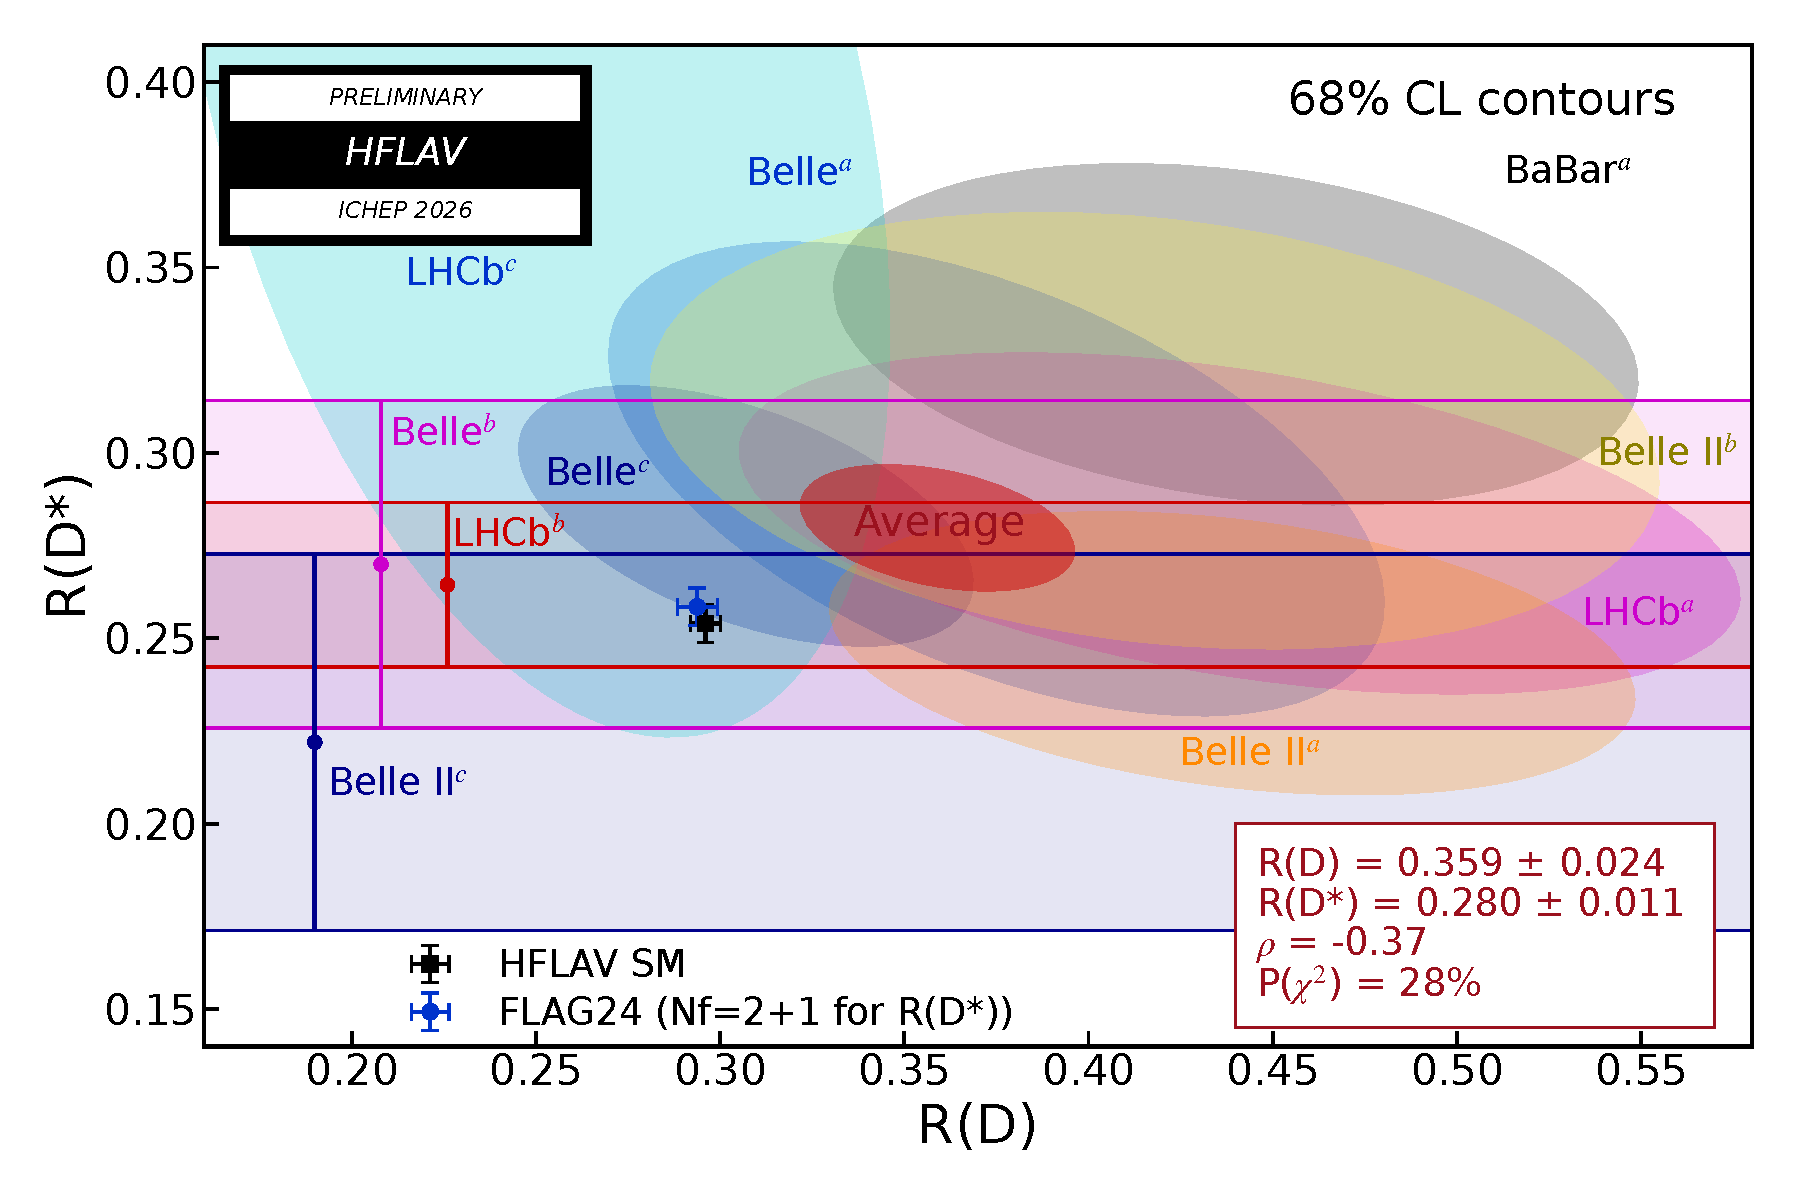
\includegraphics[width=0.75\linewidth]{Figs/CH2/rdrds_ichep_2026_prelim.pdf}
    \caption[Average of $R(D^{*})$ and $R(D)$]{Preliminary average of $R(D^{*})$ and $R(D)$ for ICHEP 2026~\cite{HFLAV2026RDstar} measured by the BaBar~\cite{BaBar:2012obs, BaBar:2013mob}, Belle~\cite{Belle:2015qfa, Belle:2016dyj, Belle:2017ilt, Belle:2019rba}, Belle-II~\cite{Belle-II:2026nmn, Belle-II:2025yjp, Shi:2026pau}, and LHCb~\cite{LHCb:2023zxo, LHCb:2023uiv, LHCb:2024jll} experiments.}
    \label{fig:HFLAV2026}
\end{figure}
\FloatBarrier


\section{Possible Solutions to the Remaining Problems of the Standard Model}
\label{sec:bsm_solutions}

Many extensions of the SM have been proposed to address one or more of the problems described above. 
This section briefly introduces several representative ideas: supersymmetry, axions, and quark--lepton unification. 
These models are not mutually exclusive, and in many cases they address different aspects of the SM's limitations.

\subsection{Supersymmetry}
\label{subsec:susy}

Supersymmetry~(SUSY) is a spacetime symmetry relating bosons and fermions~\cite{WessZumino1974,MartinSUSYPrimer}.
In supersymmetric theories, each SM particle is accompanied by a superpartner whose spin differs by one half unit.
The fermionic superpartners of bosons are conventionally named by adding the suffix `-ino', such as the gluino, wino, bino, and higgsino, while the bosonic superpartners of fermions are named by adding the prefix `s-', such as squarks and sleptons.
If supersymmetry were exact, particles and their superpartners would have equal masses.
Since no such superpartners have been observed, SUSY must be broken if it is realised in nature.

One of the main motivations for SUSY is the hierarchy problem.
Loop corrections to the Higgs mass from SM particles can be cancelled by corresponding contributions from their superpartners, reducing the sensitivity of the electroweak scale to very high energy scales~\cite{DimopoulosGeorgi1981}.
In models with conserved $R$-parity, supersymmetric particles are produced in pairs and the lightest supersymmetric particle~(LSP) is stable~\cite{FarrarFayet1978}.
If the LSP is electrically neutral and weakly interacting, such as a neutralino in many SUSY scenarios, it can provide a dark matter candidate~\cite{Goldberg1983,EllisOliveSantosoSpanos1984}.
SUSY can also improve the unification of gauge couplings at high energy, since the additional superpartners modify the renormalisation-group evolution of the gauge couplings~\cite{DimopoulosRabyWilczek1981,Amaldi1991}.
However, no direct evidence for supersymmetric particles has yet been observed, and the simplest low-scale SUSY scenarios are increasingly constrained by collider searches~\cite{ATLAS2024SUSYSummary}.

\subsection{Axions and the strong CP problem}
\label{subsec:axion}

The Peccei--Quinn mechanism provides a dynamical solution to the strong CP problem~\cite{PecceiQuinn1977PRL,PecceiQuinn1977PRD}. 
It introduces a new global chiral symmetry, usually denoted as the Peccei--Quinn symmetry $U(1)_{\mathrm{PQ}}$, which is spontaneously broken.
The associated pseudo-Nambu--Goldstone boson is the axion~\cite{Weinberg1978Axion,Wilczek1978Axion}. 
The axion field dynamically relaxes the effective value of $\bar{\theta}$ to zero, thereby explaining the absence of observable strong CP violation. 
In many models, axions or axion-like particles can also contribute to the dark matter density of the universe~\cite{KimCarosi2010}.

\subsection{Quark--lepton unification and leptoquarks}
\label{subsec:leptoquarks_motivation}

In the SM, quarks and leptons belong to separate gauge multiplets.
To unify the two sectors, the Pati--Salam framework extends the colour symmetry from $SU(3)_C$ to $SU(4)$, treating leptons as a fourth colour~\cite{PatiSalam1974}.
The additional gauge bosons that connect quarks and leptons are leptoquarks, hypothetical bosons that couple directly to a quark and a lepton.
These quark--lepton interactions allow leptoquarks to contribute to semileptonic $B$-meson decays, providing a possible explanation for the flavour anomalies discussed in Section~\ref{subsec:flavour_anomalies}.
Since couplings to the first two generations are tightly constrained by flavour measurements, a leptoquark light enough to affect $B$-meson decays has to couple mainly to the third generation, whereas the minimal Pati--Salam leptoquark couples with equal strength to all generations.

The ``4321'' model realises this flavour structure by placing only the third family in $SU(4)$ multiplets of the extended gauge group $\mathcal{G}_{4321}=SU(4)\times SU(3)'\times SU(2)_L \times U(1)'$.
After spontaneous symmetry breaking to the SM gauge group, the vector singlet leptoquark $U_{1}$ appears as a massive gauge boson coupled mainly to third-generation fermions.
For phenomenological studies, the $U_1$ leptoquark can be described by a simplified model parametrised by the leptoquark mass and its couplings to SM particles.
The 4321 model is therefore an example of an ultraviolet (UV) completion of the simplified model~\cite{Cornella2019}.

The $U_1$ interactions that contribute to $b\rightarrow c\tau\nu$ can also be probed in collider searches for final states containing hadronically decaying $\tau$ leptons.
Further discussion is given in Chapter~\ref{chapter:LQ_search}.
